\documentclass[xcolor=table]{beamer}
\usetheme{CambridgeUS}

\usepackage[utf8]{inputenc}
\usepackage[T1]{fontenc}
\usepackage[brazil]{babel}
\usepackage{amsmath}
\usepackage{amsfonts}
\usepackage{amssymb}
\usepackage{graphicx}
\usepackage{booktabs}
\usepackage{adjustbox}
\usepackage{multirow}

\author{Bruno Ferrari Guide}
\title{N-gramas e o acento no Português Brasileiro}
%\subtitle{}
%\logo{}
\institute{Orientador: Marcelo Barra Ferreira\\ Departamento de Linguística - FFLCH - USP}
\date{12 de abril de 2015}
%\subject{}
%\setbeamercovered{transparent}
%\setbeamertemplate{navigation symbols}{}

\begin{document}
	%1
	\maketitle
%%%%%%%%%%%%%%%%%%%%%%%%%%%%%%%%%%%%%%%%%%
	\section{Introdução}
	%2
	\begin{frame}
		\frametitle{Introdução}
		\begin{itemize}
			\item Tópicos dessa apresentação:\\
			\begin{itemize}
				\item Objetivos\\
				\item Sobre o acento\\
				\item Modelos de N-Gramas\\
				\item Resultados\\
				\item Perspectivas\\
			\end{itemize}
		\end{itemize}
	\end{frame}

%%%%%%%%%%%%%%%%%%%%%%%%%%%%%%%%%%%%%%%%%%%%%

	\section{Objetivos}
	%3
	\begin{frame}
		\frametitle{Objetivos}
		\begin{itemize}
			\item A partir da criação de modelos probabilísticos, eu pretendo apresentar uma discussão sobre o comportamento do acento no PB.\\
			\item Os modelos são baseados em corpus e podem trazer à tona algumas características quantitativas sobre esse comportamento.\\
			\item Os modelos retornam as probabilidades de uma determinada palavra pertencer a alguma categoria acentual (Oxítona, Paroxítona, Proparoxítona) e a partir disso é possível discutir os erros e os acertos de um modelo.\\
		\end{itemize}
	\end{frame}


%%%%%%%%%%%%%%%%%%%%%%%%%%%%%%%%%%%%%%%%%%%%%

	\section{Sobre o Acento}
	\begin{frame}
		\centering \textbf{Sobre o acento\\}
	\end{frame}
	%4
	\begin{frame}
		\frametitle{Sobre o Acento - 2 tendências}
		\begin{itemize}
			\item O acento no português brasileiro (quase) sempre ocupa uma das três últimas posições da palavra, criando as três categorias acentuais: Oxítona, Paroxítona, Proparoxítona.
			\item Duas tendências dão conta da maioria das palavras do PB:
			\begin{itemize}
				\item Caso a sílaba final seja pesada, a palavra é oxítona.\\
				\item Caso a sílaba final seja leve, a palavra é paroxítona.\\
			\end{itemize}
		\end{itemize}
	\end{frame}
	%5
	\begin{frame}
		\frametitle{2 tendências?}
		\begin{itemize}
			\item Problemas com palavras oxítonas terminadas em sílaba leve, como \textit{caqui, urubu}\\
			\item Problemas com paroxítonas terminadas em sílaba pesada, como em \textit{mártir, câncer, difícil}.\\
			\item Problemas com as proparoxítonas de modo geral.\\
			\item O acento é regular, porém tem irregularidades.\\
			\item O acento é irregular, porém tem regularidades.\\
		\end{itemize}

	\end{frame}	
%%%%%%%%%%%%%%%%%%%%%%%%%%%%%%%%%%%%%%%%%%%%%%%%%%%%%
	\section{Modelos de N-Gramas}
	
	\begin{frame}
		\centering \textbf{Modelos de N-Gramas\\}
	\end{frame}
	
	\begin{frame}
		\frametitle{Sobre modelos probabilísticos}
		\begin{itemize}
			\item Modelo é uma representação formal de um objeto.\\
			\item As vezes, o objeto possui comportamento imprevisível.\\
			\item Na matemática, a área que lida com a imprevisibilidade (ou seja, que a quantifica e formaliza) é a probabilidade.\\
			\item Existem muitas formas de tentar formalizar essa imprevisibilidade, cada uma possui suas vantagens e desvantagens.\\
		\end{itemize}
	\end{frame}
	%6
	\begin{frame}
		\frametitle{Modelos de N-Gramas: princípios}
		\begin{itemize}
			\item A noção de língua subjacente é simples.\\
			\item Poderíamos atribuir probabilidade levando em conta a palavra inteira.\\
			\item Mas a ideia é que se pode atribuir à sequência a sua probabilidade a partir da probabilidade condicional não dela inteira, mas somente da sequências de tamanho N que a compõe. (Cadeia de Markov de tamanho N).\\ 
		\end{itemize}
		{\small P(X$_{i+1}$=x$\mid$ X$_{1}$=x$_{1}$,X$_{2}$=x$_{2}$,$\ldots$ ,X$_{i}$=x$_{i}$)=P(X$_{i+1}$=x$\mid$ X$_{i}$=x$_{i}$ $\ldots$ X$_{i-N}$=x$_{i-N}$) }
	\end{frame}
	
		\begin{frame}
			\frametitle{Funcionamento do modelo para a questão do acento}
			\begin{itemize}
				\item Se atribui uma probabilidade a partir do modelo para cada uma das versões acentuadas de uma palavra a partir das frequências extraídas do Corpus.\\
				\item A palavra é quebrada nos n-gramas que a compõe e a probabilidade final é o produto das probabilidades dos n-gramas que a compõe.\\
				\item Ex: (num modelo de bi-gramas)
				\begin{itemize}
					\item P(\&\textbf{es}trela*) = P(\textbf{e}$\mid$\&)* P(\textbf{s}$\mid$\textbf{e})* P(t$\mid$\textbf{s})...\\
					\item P(\&es\textbf{tre}la*) = P(e$\mid$\&)* P(s$\mid$e)* P(t$\mid$s)...\\
					\item P(\&estre\textbf{la}) = P(e$\mid$\&)* P(s$\mid$e)* P(t$\mid$s)...\\
					a partir da noção de que:\\
					\item P(e$\mid$\&) = $\dfrac{C(\&e)}{C(\&)}$
				\end{itemize}
			\end{itemize}
		\end{frame}
	
	%7
	\begin{frame}
		\frametitle{Modelos de N-Gramas: Entrada}
		\begin{itemize}
		\item O modelo recebe como entrada uma palavra transcrita.\\
		\item A transcrição foi feita automaticamente.\\
		\item O corpus utilizado é o Corpus ABG, compilado em conjunto com a colega Aline Benevides.\\
		\item As palavras monossílabas foram descartadas para essa pesquisa.\\
		\item Com isso, o corpus tem cerca de 95 mil tipos de palavras diferentes.\\
		
		\end{itemize}	
	\end{frame}
	
	%8		

	%9
	\begin{frame}
		\frametitle{Diferentes Modelos: Tamanho de N}
		\begin{itemize}
			\item Quanto maior a cadeia de n-gramas, mais complexo e informativo é o modelo.\\
			\item Quanto maior a cadeia, maior o número de possíveis n-gramas:\\
			\begin{quote}
				\centering C = $\alpha^n$ 
			\end{quote}
			\item Com mais possibilidades, é necessário um Corpus cada vez maior para o modelo funcionar.\\
			\item Por isso, os tamanhos de n escolhidos foram 2 (bi-gramas) e 3 (tri-gramas).\\
		\end{itemize}
	\end{frame}
	%10
	\begin{frame}
		\frametitle{Diferentes Modelos: Tipos e Ocorrências}
		\begin{itemize}
			\item O modelo baseado em tipos contabiliza toda palavra uma única vez.\\
			\item O modelo baseado em ocorrências inclui as repetições de uma mesma palavra.\\
			\item O corpus ABG já contem esse tipo de informação.\\
			\item No entanto, uma vez que foram eliminadas as palavras monossílabas, o comportamento do acento em termos quantitativos tanto nos tipos quanto nas ocorrências ficou bastante similar.\\
		\end{itemize}
	\end{frame}	
	%11
	\begin{frame}
		\frametitle{Diferentes Modelos: Conhecimento embutido}
		\begin{itemize}
			\item Caso a probabilidade atribuída pelo modelo de n-gramas resulte em um empate entre duas palavras candidatas, qual medida tomar?\\
			\item Nos modelos sem heurística, tal situação foi considerada um erro.\\
			\item Nos modelos com heurística, o modelo escolhia uma das candidatas empatadas. No caso, a que pertencesse a uma das categorias mais comum.\\
			\item (Paroxítona > Oxítona > Proparoxítona)\\
		\end{itemize}
	\end{frame}
	%12
	\begin{frame}
		\frametitle{Modelos de N-Gramas e a linguistica: Bigramas}
		% Please add the following required packages to your document preamble:
		% \usepackage{booktabs}
			\centering
			\adjustbox{max height=\dimexpr\textheight-5.5cm\relax,
				max width=\textwidth}{
			\label{TAB1}
			\begin{tabular}{@{}llll@{}}
				\textbf{r} &        &     &       \\ \midrule
				& tokens &     & types \\ \cmidrule(l){2-4} 
				-r         & 238189 & -r  & 15433 \\
				r-         & 128499 & r-  & 8181  \\
				ra         & 125610 & ra  & 5914  \\
				r*         & 120046 & rE  & 4218  \\
				1r         & 69086  & r*  & 4215  \\
				\textbf{p} &        &     &       \\ \midrule
				\&p        & 215256 & -p  & 8563  \\
				-p         & 110325 & \&p & 6715  \\
				pr         & 64697  & pr  & 3347  \\
				pe         & 48205  & pe  & 3140  \\
				pa         & 40335  & pa  & 2360  \\ \bottomrule
			\end{tabular}
		}
	\end{frame}
	%13
	\begin{frame}
		\frametitle{Modelos de N-Gramas e a linguistica Trigramas}
		\centering
		\adjustbox{max height=\dimexpr\textheight-5.5cm\relax,
			max width=\textwidth}{
			\label{TAB2}
			\begin{tabular}{@{}llll@{}}
				\textbf{r} &        &      &       \\ \midrule
				& tokens &      & types \\ \midrule
				-ra        & 84376  & a-r  & 3587  \\
				rA*        & 77924  & ra-  & 3448  \\
				1r*        & 60944  & -ra  & 3231  \\
				\&pr       & 48882  & re-  & 2999  \\
				-tr        & 48243  & e-r  & 2715  \\
				\textbf{p} &        &      &       \\ \midrule
				\&pr       & 48882  & pE-  & 2175  \\
				pE-        & 36883  & \&pr & 2078  \\
				\&p1       & 36340  & -pE  & 1884  \\
				\&pE       & 31120  & pa-  & 1732  \\
				p1-        & 28943  & A-p  & 1721 
			\end{tabular}
		}
	\end{frame}		
	%14
	\begin{frame}
		\frametitle{Diferentes Modelos: Segmento e Sílaba}
		\begin{itemize}
			\item Montei uma versão do corpus só com palavras com 3 sílabas ou mais.\\
			\item O que alimenta o modelo não são os segmentos, e sim as sílabas.\\
			\item A palavra 'pedrada' seria representada em bigramas da seguinte maneira então:  ['pe-dra','dra-da']\\
			\item Expectativa de que os resultados fossem bastante interessantes, dado que é um modelo muito informativo.\\
		\end{itemize}
	\end{frame}	
%%%%%%%%%%%%%%%%%%%%%%%%%%%%%%%%%%%%%%%%%%%%%%
	\section{Resultados}
	\begin{frame}
		\centering \textbf{Resultados}
	\end{frame}
	%15
	\begin{frame}
		\frametitle{Obtendo os resultados}
		A metodologia para a obtenção dos resultados foi a seguinte:
		\begin{itemize}
			\item O processo começa com a separação randômica do corpus entre corpus treino (80$\%$) e corpus teste (20$\%$).\\
			\item O corpus treino alimenta o modelo.\\ 
			\item O modelo atribui probabilidades às diferentes versões acentuadas das palavras do corpus teste.\\
			\item A probabilidade mais alta para cada candidata é escolhida, a partir disso se compara com a acentuação correta da palavra.\\
			\item O modelo acerta se a categoria que elegeu mais provável é a categoria da qual a palavra faz parte.\\
			\item Esse processo foi repetido 100 vezes para cada modelo.\\
		\end{itemize}
	\end{frame}
	%16
	\begin{frame}
		\frametitle{Resultados N-Gramas}
		\begin{figure}
\centering
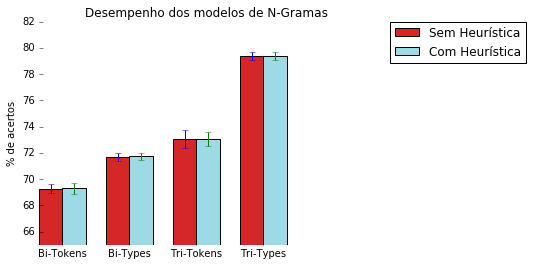
\includegraphics[width=0.7\linewidth]{desempenhoN-gramas}
\caption{Desempenho dos modelos de N-gramas}
\label{fig:desempenhoN-gramas}
\end{figure}

	\end{frame}	
	%17
	\begin{frame}
		\frametitle{Análise N-Gramas baseado em segmentos}
		\centering
		\label{TAB3}
		\begin{tabular}{@{}llcc@{}}
			\textbf{Modelos}                  &       & \textbf{Media Acertos} & \textbf{Desvio Padrão}  \\ \midrule
			\multirow{2}{*}{Bi-tok}  & Sem H & 69.29 & 0.36 \\ \cmidrule(l){2-4} 
			& Com H & 69.30 & 0.43 \\ \midrule
			\multirow{2}{*}{Bi-typ}  & Sem H & 71.69 & 0.30 \\ \cmidrule(l){2-4} 
			& Com H & 71.74 & 0.28  \\ \midrule
			\multirow{2}{*}{Tri-tok} & Sem H & 73.05 & 0.66 \\ \cmidrule(l){2-4} 
			& Com H & 73.05 & 0.54 \\ \midrule
			\multirow{2}{*}{Tri-typ} & Sem H & 79.40 & 0.30 \\ \cmidrule(l){2-4} 
			& Com H & 79.38 & 0.27
		\end{tabular}
	\end{frame}
	%18
	\begin{frame}
		\frametitle{Resultados Sílabas}
\begin{figure}
\centering
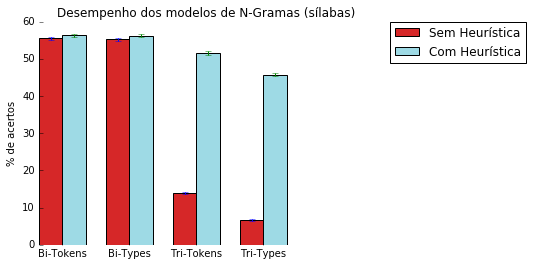
\includegraphics[width=0.7\linewidth]{desempenhoN-gramas-sil}
\caption{Desempenho dos modelos de N-gramas baseados em Sílaba.}
\label{fig:desempenhoN-gramas-sil}
\end{figure}

	\end{frame}	
	%19
	\begin{frame}
		\frametitle{Análise N-Gramas baseados em sílabas}
		\centering
		\label{TAB4}
		\begin{tabular}{@{}llcc@{}}
			\textbf{Modelos}                    &  & \textbf{Média de Acertos} & \textbf{Desvio Padrão} \\ \midrule
			\multirow{2}{*}{Bigramas (Tokens)}  & Sem H                        & 55.53                     & 0.43                   \\ \cmidrule(l){2-4} 
			& Com H                        & 56.31                     & 0.39                   \\ \midrule
			\multirow{2}{*}{Bigramas (Types)}   & Sem H                        & 55.24                     & 0.39                   \\ \cmidrule(l){2-4} 
			& Com H                        & 56.22                     & 0.35                   \\ \midrule
			\multirow{2}{*}{Trigramas (Tokens)} & Sem H                        & 13.96                     & 0.25                   \\ \cmidrule(l){2-4} 
			& Com H                        & 51.54                     & 0.42                   \\ \midrule
			\multirow{2}{*}{Trigramas (Types)}  & Sem H                        & 6.72                      & 0.19                   \\ \cmidrule(l){2-4} 
			& Com H                        & 45.75                     & 0.42                  
		\end{tabular}
	\end{frame}
	
	%20
	\begin{frame}
		\frametitle{Resultados Gerais}
		\begin{figure}
\centering
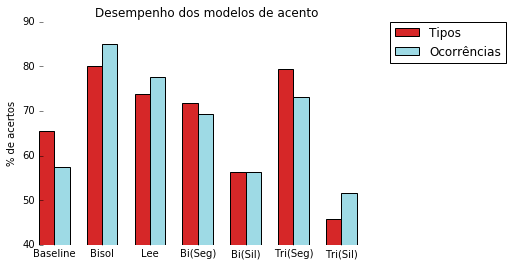
\includegraphics[width=0.7\linewidth]{desempenhoN-gramas-geral}
\caption{Desempenho dos modelos de N-gramas em comparação com os modelos baseados em Lee (1995), Bisol (1992) e o Baseline.}
\label{fig:desempenhoN-gramas-geral}
\end{figure}

	\end{frame}	
%%%%%%%%%%%%%%%%%%%%%%%%%%%%%%%
	\section{Perspectivas}
	%22
	\begin{frame}
		\frametitle{Próximos passos}
		\begin{itemize}
			\item Implementar outro modelo probabilístico, que leva em conta dados linguísticos além da frequência dos segmentos. No caso, o modelo a ser implementado será o Classificador Bayesiano Ingênuo.\\
			
			\item Escrever, escrever, escrever...
		\end{itemize}
	\end{frame}
	%23
	\begin{frame}
		\frametitle{Agradecimento}
		Muito Obrigado!
		
	\end{frame}
\end{document}